%**************************************************************
% Lab 13: Elevator
%**************************************************************
\chapter{Elevator}

\section{Purpose}

This final lab is used as a capstone digital logic project. 

\section{Challenge}

For this lab, build a circuit that simulates an elevator. This lab does not include step-by-step directions; instead, this document only specifies the requirement and students are on their own to design and build the circuit.

Here are the specifications:

\begin{enumerate}
	\item The elevator should be in a 3-story building and stop on each floor.
	\item There should be a call button on each floor so a guest can request the elevator. When a guest presses the call button, if the elevator is not busy, then it should proceed to the requested floor. If the elevator is busy, it should return to the called floor as soon as it finishes the current trip.
	\item The elevator car must have a button for each floor (for this lab, ignore buttons like ``Open Door''). When one of the buttons is pressed, the elevator will move to the requested floor. If the elevator is already on the requested floor (for example, some guest on the second floor presses the ``Floor 2'' button), then the elevator will do nothing.
	\item The simulator must have some way to indicate where the elevator is located (its current floor). That could be done with a numeric display (a 7-segment display) or with some sort of light system (an LED on each floor that will light up when the elevator is present). There may be other ways to indicate the elevator's location, so creativity is encouraged.
	\item The simulator must have some way to indicate the ``door open'' and ``door close'' process. For example, a row of LEDs could light in sequence to show the door opening and a few seconds later closing again.
\end{enumerate}

Figure \ref{fig:13-01} is one student's concept from an earlier class. 

\begin{figure}[H]
	\centering
	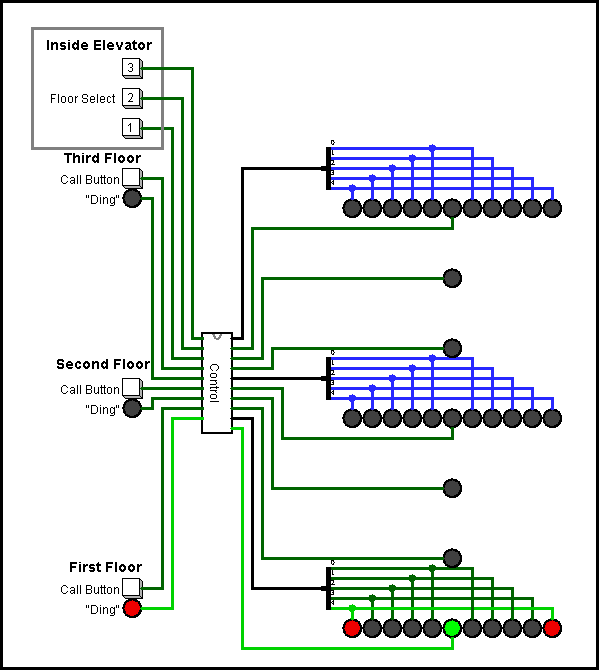
\includegraphics[width=\maxwidth{.95\linewidth}]{gfx/13-01}
	\caption{Example Elevator Simulator}
	\label{fig:13-01}
\end{figure}

\section{Deliverable}

To receive a grade for this lab, complete the elevator simulator. Be sure the standard identifying information is at the top left of the \lstinline{main} circuit: 

\bigskip
% The minipage environment keeps the three lines together - no page break.
\begin{minipage}{\linewidth}
	\begin{verbatim}
	George Self
	Lab 12: Elevator
	April 30, 2018
	\end{verbatim}
\end{minipage}
\bigskip

Save the file with this name: \textit{Lab12\_elevator} and submit that file for grading.